
%(BEGIN_QUESTION)
% Copyright 2006, Tony R. Kuphaldt, released under the Creative Commons Attribution License (v 1.0)
% This means you may do almost anything with this work of mine, so long as you give me proper credit

En tank med prosessvæske trenger nivåovervåking.  Nivåområdet i tanken er 0 til 3 meter, og prosessvæsken har tetthet 1000 kg/m$^3$, lik vann.  Noen velger å montere en trykktransmitter i bunnen av tanken for å beregne nivå ut fra hydrostatisk trykk, slik:

$$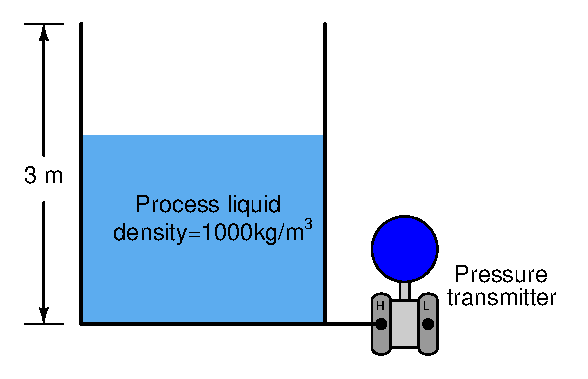
\includegraphics[width=15.5cm]{i00248x01.eps}$$

Senere monteres et lokk på tanken for å hindre regnvann i å komme inn.  Dessverre avgir prosessvæsken damp som blir fanget i den lukkede tanken og skaper overtrykk.  En liten ventil monteres på toppen for å slippe ut damp, men ventilen er {\it liten}, ikke stor nok til å sikre fullstendig fravær av damptrykksoppbygging til enhver tid:

$$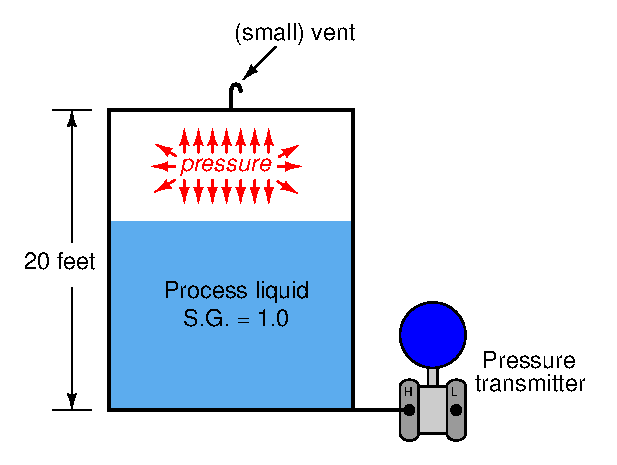
\includegraphics[width=15.5cm]{i00248x02.eps}$$

Hvilket måleproblem oppstår når det av og til bygges opp damptrykk i denne tanken?  Hvordan kan problemet korrigeres slik at væskenivået måles riktig til enhver tid?

\underbar{file i00248}
%(END_QUESTION)





%(BEGIN_ANSWER)

Ethvert damptrykk vil registreres av transmitteren og tolkes som økt væskenivå.

\vskip 10pt

To løsninger på dette problemet:

\vskip 10pt {\narrower \noindent \baselineskip5pt

(1) Bruk to transmittere (én på tanktoppen, én på tankbunnen) og subtraher utgangssignalene elektronisk.

\par} \vskip 10pt



\vskip 10pt {\narrower \noindent \baselineskip5pt

(2) Koble ``lav''-siden på én $\Delta$P-transmitter til toppen av tanken for naturlig kompensasjon av damptrykket.

\par} \vskip 10pt

Siden transmitteren beregner nivå ut fra trykket i bunnen av tanken, vil ethvert oppbygget damptrykk i tanken bli feiltolket som ekstra væskenivå, fordi transmitteren måler {\it summen} av hydrostatisk trykk og fanget damptrykk.

For eksempel: hvis væskenivået er 10 fot (50\% av området), vil hydrostatisk trykk fra væskesøylen være 120 inches W.C., forutsatt spesifikk vekt 1.0 (som vann).  Hvis tanken samtidig har damptrykk lik 15 inches W.C., legges dette til de 120 inches W.C. fra væskehodet og gir totalt 135 inches W.C. målt trykk.  Resultatet er at transmitteren ``tror'' nivået er 11.25 fot (135 tommer) i stedet for faktisk 10 fot (120 tommer).  I praksis gir damptrykk i tanken et ``nullpunktskift'' i transmitterindikasjonen.

I mange applikasjoner er gasstrykket i tanken langt høyere enn hydrostatisk trykk fra væskesøylen, så problemet kan være svært alvorlig i nivåmåling.  Vi må forstå problemet fullt ut og hvordan det løses for å måle nivå riktig i mange industrielle prosesser.

Løsningen er å måle {\it trykkforskjellen} mellom topp og bunn i tanken.  Dette kan gjøres med to trykktransmittere (én på toppen og én på bunnen), der hydrostatisk trykk bestemmes ved å subtrahere topptransmitterens måling fra bunntransmitterens måling.  En datamaskin kan gjøre signal-subtraksjonen:

$$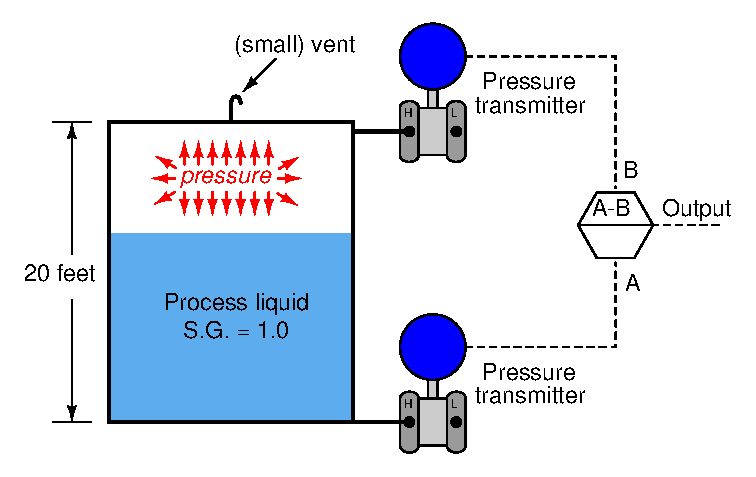
\includegraphics[width=15.5cm]{i00248x03.eps}$$

En annen, mer elegant metode er å bruke en {\it differanse}trykktransmitter med rørtilkobling til begge ender av tanken.  Denne løsningen utfører subtraksjonen mekanisk ved å eksponere føler-elementet direkte for {\it differansen} mellom to trykk:

$$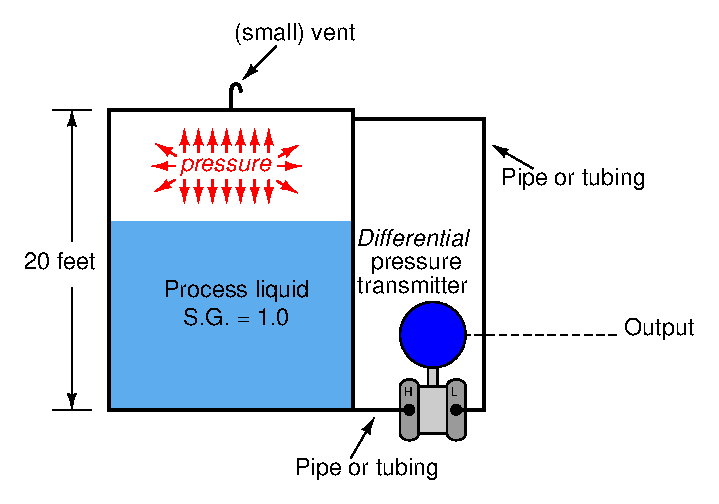
\includegraphics[width=15.5cm]{i00248x04.eps}$$

Fordi differansetrykkløsningen krever bare ett måleinstrument i stedet for to, og gir bedre nøyaktighet siden vi kun håndterer unøyaktigheten i ett instrument (ikke summerte feil fra to instrumenter, eventuelt tre med en separat subtraksjonsenhet), er differanse- eller ``d/p''-løsningen den mest brukte.

I denne konkrete nivåapplikasjonen vil et differansetrykkinstrument ha nøyaktig samme kalibreringspunkter (nedre og øvre måleverdi) som en ``vanlig'' trykktransmitter tilkoblet en åpen tank.

%(END_ANSWER)





%(BEGIN_NOTES)


%INDEX% Measurement, level: hydrostatic pressure + vapor pressure compensation

%(END_NOTES)
